\section{Chapter one}

\vspace*{\fill}

\begin{example}
  \centering
  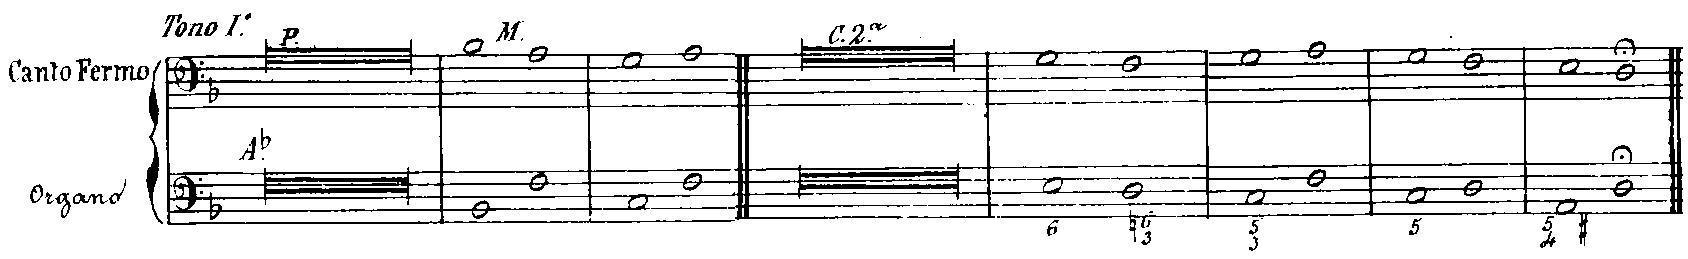
\includegraphics[width=\linewidth]{c/1/ex/alfieri_tone2_5long.jpg}
  \vspace*{2em}
  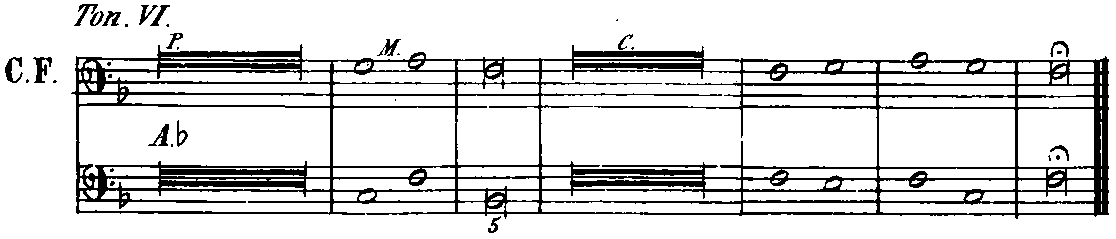
\includegraphics[width=.8\linewidth]{c/1/ex/alfieri_tone6_7long.png}
  \caption{Alfieri, Reputedly antiquated psalm-tone basses}
  \label{mus:alfieri_antiquated}
\end{example}

\vspace*{\fill}

\newpage

\vspace*{\fill}

\begin{example}
  \centering
  \includegraphics[width=\linewidth]{c/1/ex/antonio_christe_2.png}
  \caption{António, Considerable inner part movement, 1761}
  \label{mus:antonio_christe}
\end{example}

\vspace*{\fill}

\begin{example}
  \centering
  \includegraphics[width=\linewidth]{c/1/ex/knecht_vol3_60.png}
  \caption{Knecht, Harmonisation in the second mode, 1798}
  \label{mus:knecht_secondmode}
\end{example}

\vspace*{\fill}

\begin{landscape}

  \vspace*{\fill}

  \begin{example}
    \centering
    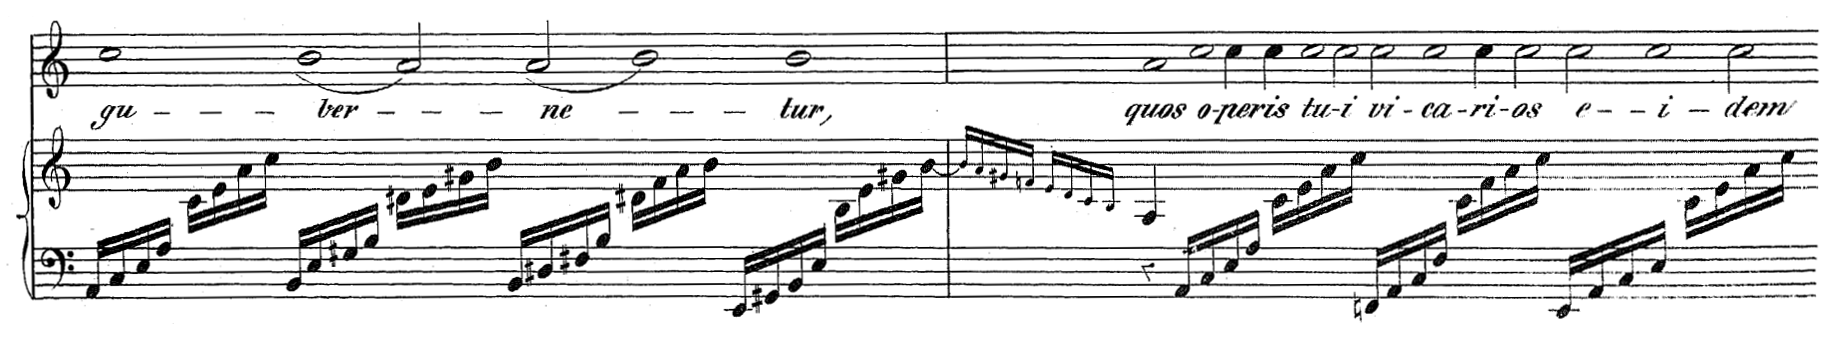
\includegraphics[width=\linewidth]{c/1/ex/neubig_arpeggio_36.png}
    \caption{Neubig, `arpeggio Begleitung', 1844}
    \label{mus:neubig_arpeggio}
  \end{example}

  \vspace*{\fill}

  \begin{example}
    \centering
    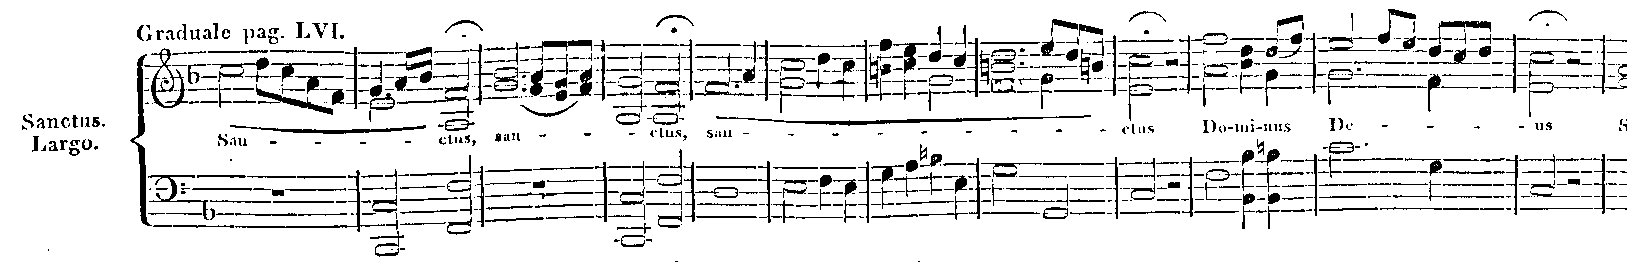
\includegraphics[width=\linewidth]{c/1/ex/jar_sanctus_55.png}
    \caption{Jarmusiewicz, Ornamented accompaniment, 1834}
    \label{mus:jar_sanctus_55}
  \end{example}

  \vspace*{\fill}

\end{landscape}

\vspace*{\fill}

\begin{example}
  \centering
  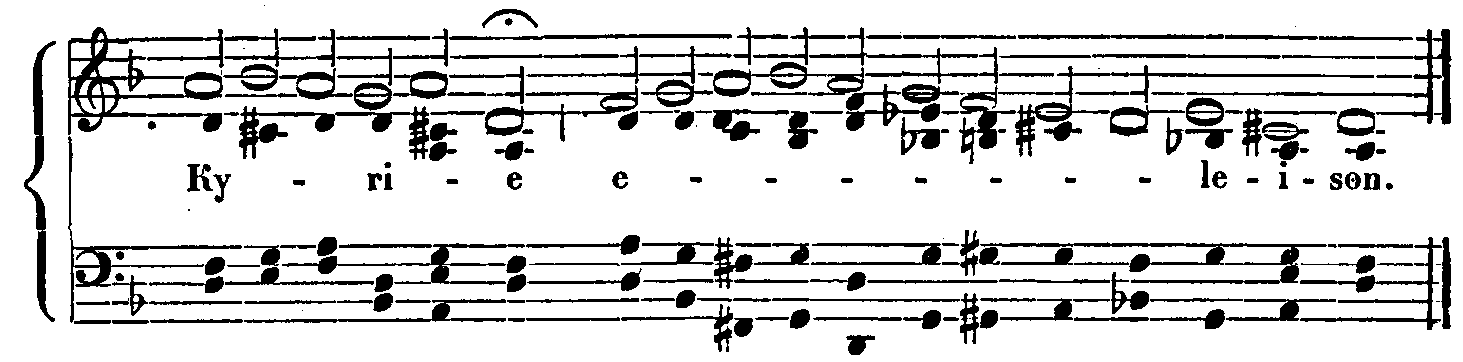
\includegraphics[width=\linewidth]{c/1/ex/wincenty.png}
  \caption{Gor\k{a}czkiewicz, Neapolitan and diminished harmonies, 1847}
  \label{mus:wincenty}
\end{example}

\vspace*{\fill}

\begin{example}
  \centering
  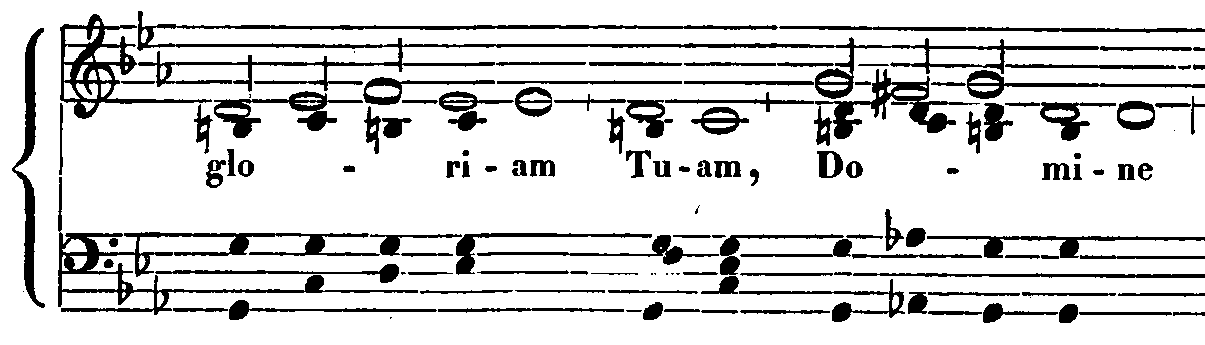
\includegraphics[width=.9\linewidth]{c/1/ex/wincentysixth.png}
  \caption{Gor\k{a}czkiewicz, French sixth harmony, 1847}
  \label{mus:wincentysixth}
\end{example}

\vspace*{\fill}

\newpage

\vspace*{\fill}

\begin{example}
  \centering
  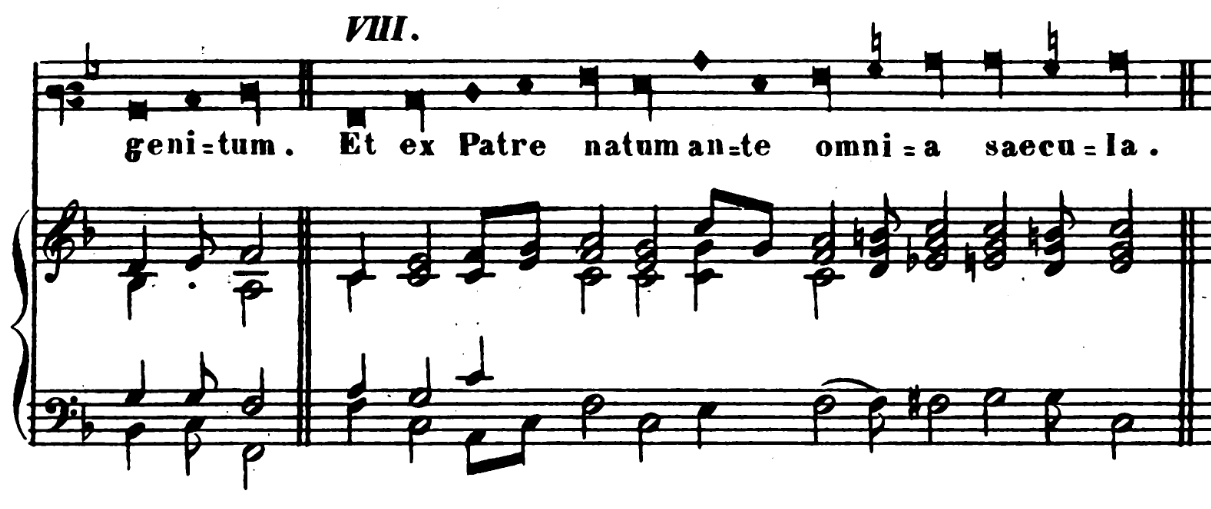
\includegraphics[width=.8\linewidth]{c/1/ex/stehlin_etexpatre_31.png}
  \caption{Stehlin, Tetrardus modulation to C major, 1842}
  \label{mus:stehlin_etexpatre_31}
\end{example}

\vspace*{\fill}

\begin{example}
  \centering
  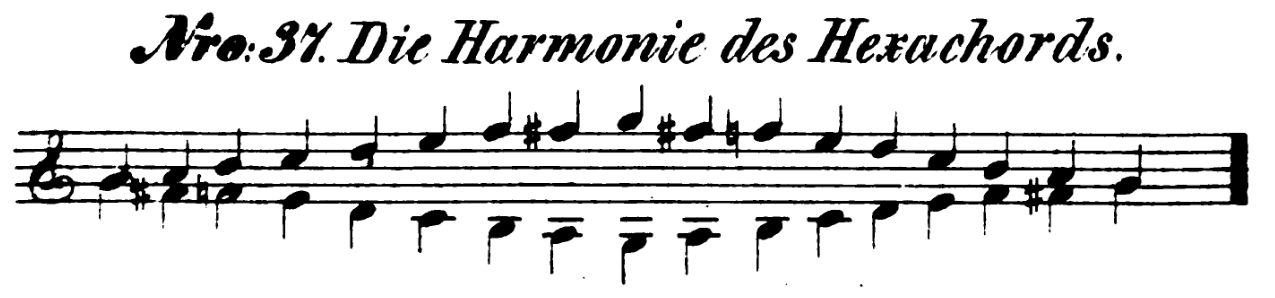
\includegraphics[width=.8\linewidth]{c/1/ex/stehlin_hexachords_54natur.png}
  \caption{Stehlin, Experimental derivation of harmony from hexachords, 1852}
  \label{mus:stehlin_hexachords_54}
\end{example}

\vspace*{\fill}

\newpage

\vspace*{\fill}

\begin{example}
  \centering
  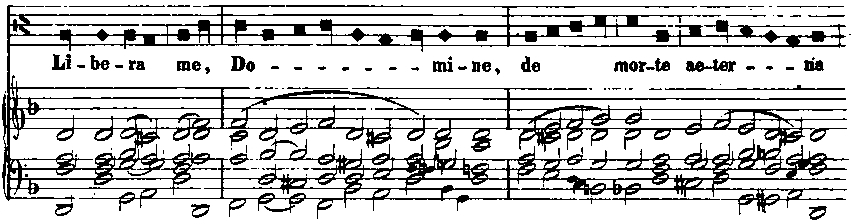
\includegraphics[width=\linewidth]{c/1/ex/homeyer_libera_113.jpg}
  \caption{Homeyer, Harmony conflicting with chant, 1846}
  \label{mus:homeyer_libera_113}
\end{example}

\vspace*{\fill}

\begin{example}
  \centering
  \includegraphics[width=\linewidth]{c/1/ex/schwarz_avemarisstella_39.png}
  \caption{Schwarz, \emph{Ibid}., 1846}
  \label{mus:schwarz_avemarisstella_39}
\end{example}

\vspace*{\fill}

\newpage

\vspace*{\fill}

\begin{example}
  \centering
  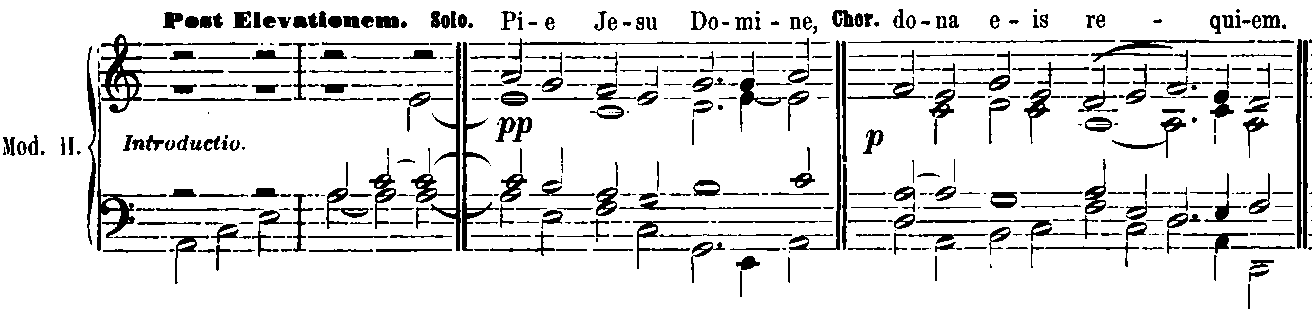
\includegraphics[width=\linewidth]{c/1/ex/schneider_piejesu_131.png}
  \caption{Schneider, Protus cadence using A minor \rightarrow{} D minor harmony, 1866}
  \label{mus:schneider_piejesu_131}
\end{example}

\vspace*{\fill}

\begin{example}
  \centering
  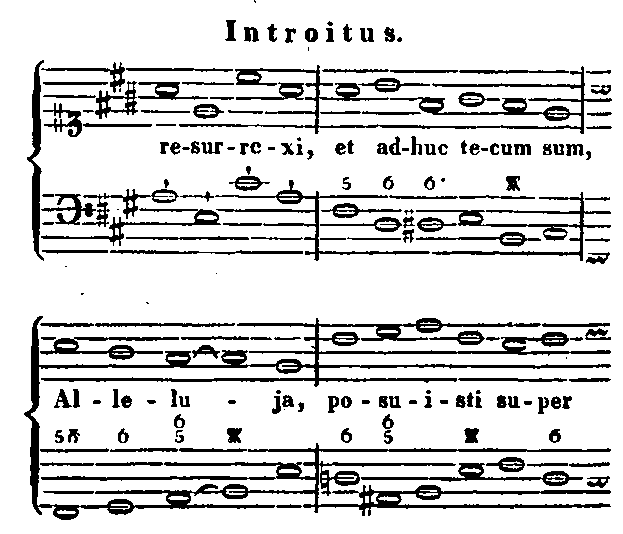
\includegraphics[width=.8\linewidth]{c/1/ex/ett_easterintroit_40.png}
  \caption{Ett, Chordal texture with bare octaves, 1834}
  \label{mus:ett_easterintroit_40}
\end{example}

\vspace*{\fill}

\newpage

\begin{landscape}

  \vspace*{\fill}

  \begin{example}
    \centering
    \includegraphics[width=.8\linewidth]{c/1/ex/benz_1850_41.png}
    \caption{Benz, Unison and SATB passages, 1850}
    \label{mus:benz_1850_41}
  \end{example}

  \vspace*{\fill}

\end{landscape}

\begin{landscape}

  \vspace*{\fill}

  \begin{example}
    \centering
    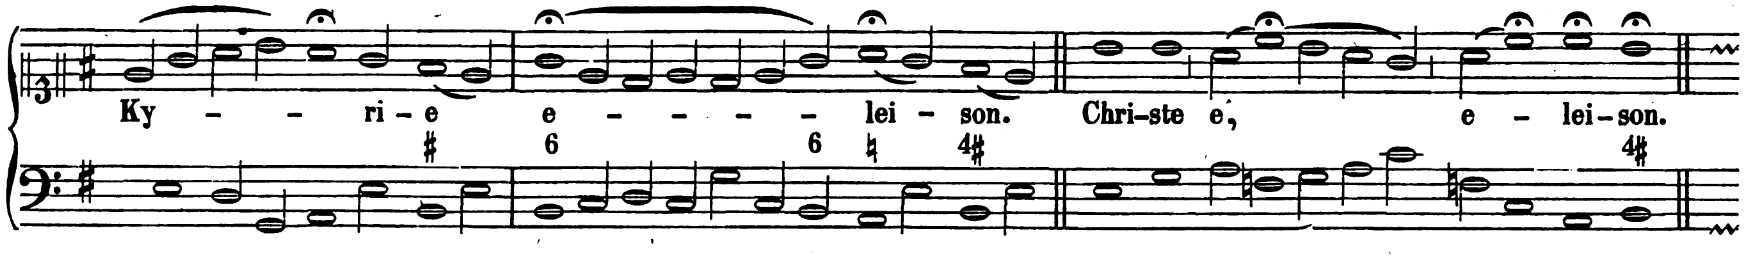
\includegraphics[width=.8\linewidth]{c/1/ex/mettenleiter_enchiridion_8.png}
    \caption{Mettenleiter, Chordal texture, 1854}
    \label{mus:mettenleiter_enchiridion_8}
  \end{example}

  \vspace*{\fill}

  \begin{example}
    \centering
    \includegraphics[width=.6\linewidth]{c/1/ex/bruckner_venicreator_524.png}
    \caption{Bruckner, Minor-mode harmonisation of `Veni creator'}
    \label{mus:bruckner_venicreator_524}
  \end{example}

  \vspace*{\fill}

\end{landscape}

\begin{landscape}

  \vspace*{\fill}

  \begin{example}
    \centering
    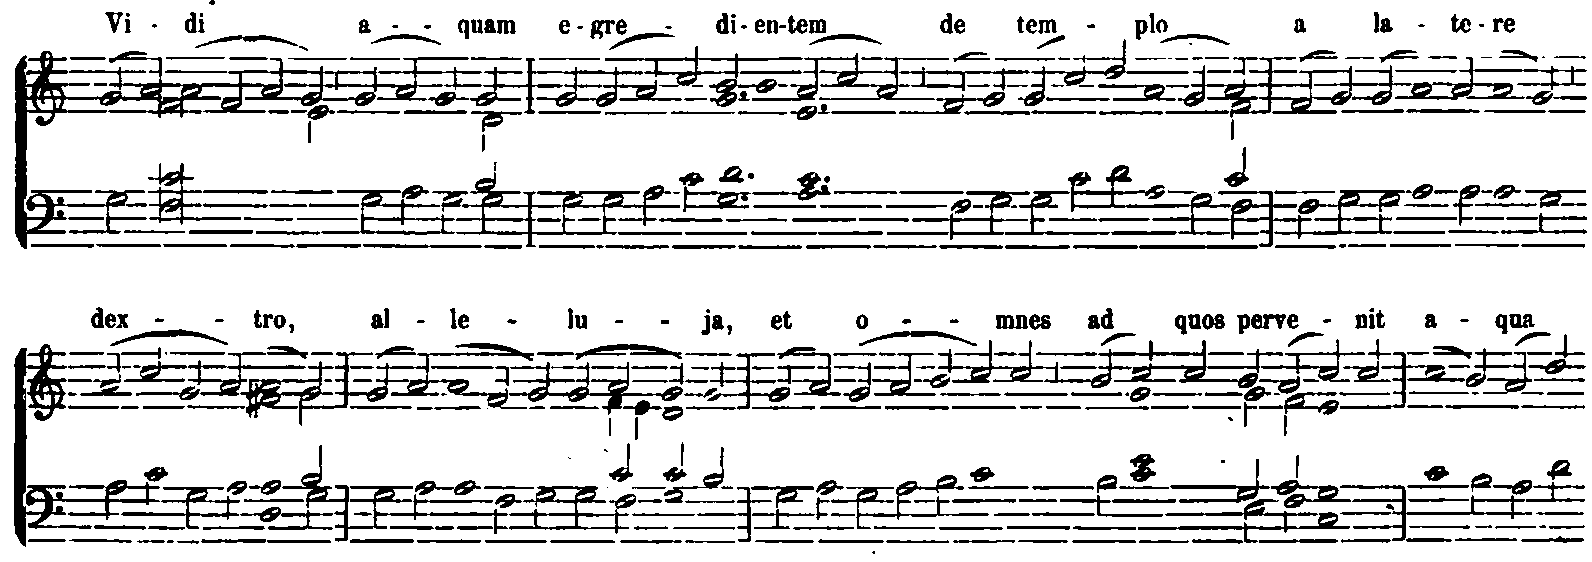
\includegraphics[width=.8\linewidth]{c/1/ex/witt_appendix.png}
    \caption{Witt, Antiquated ideal of accompaniment, 1872}
    \label{mus:witt_appendix}
  \end{example}

  \vspace*{\fill}

\end{landscape}

\begin{landscape}

  \vspace*{\fill}

  \begin{example}
    \centering
    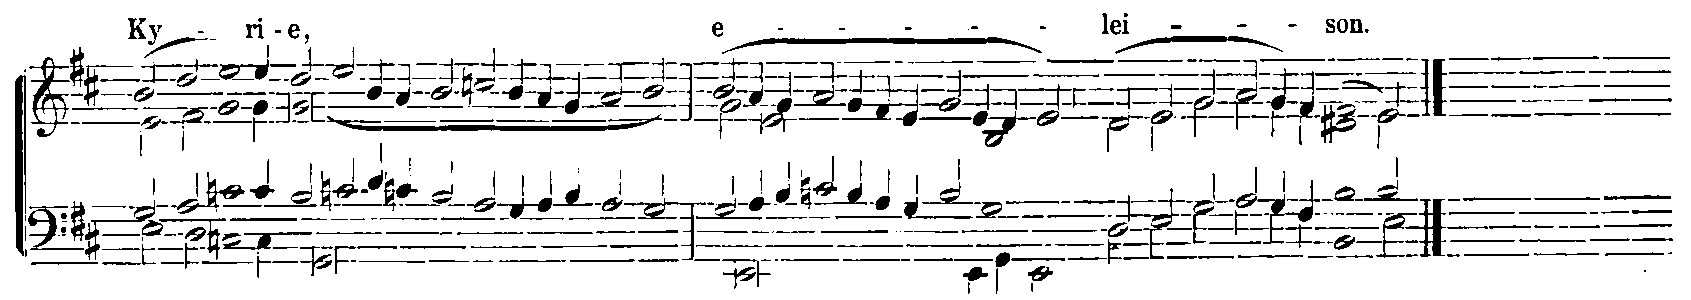
\includegraphics[width=.9\linewidth]{c/1/ex/witt_continuous_30.png}
    \caption{Witt, `Passing notes' system, 1872}
    \label{mus:witt_continuous_30}
  \end{example}

  \vspace*{\fill}

\end{landscape}

\begin{landscape}

  \vspace*{\fill}

  \begin{example}
    \centering
    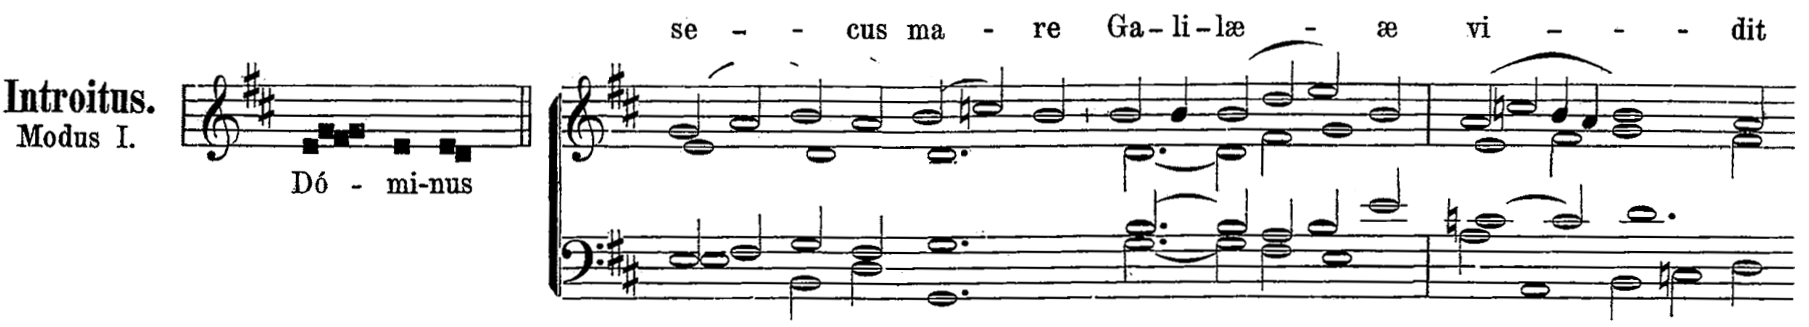
\includegraphics[width=.8\linewidth]{c/1/ex/hanisch_auxiliary_1.png}
    \caption{Hanisch, Dissonant upper auxiliary, 1883}
    \label{mus:hanisch_upper_1}
  \end{example}

  \vspace*{\fill}

  \begin{example}
    \centering
    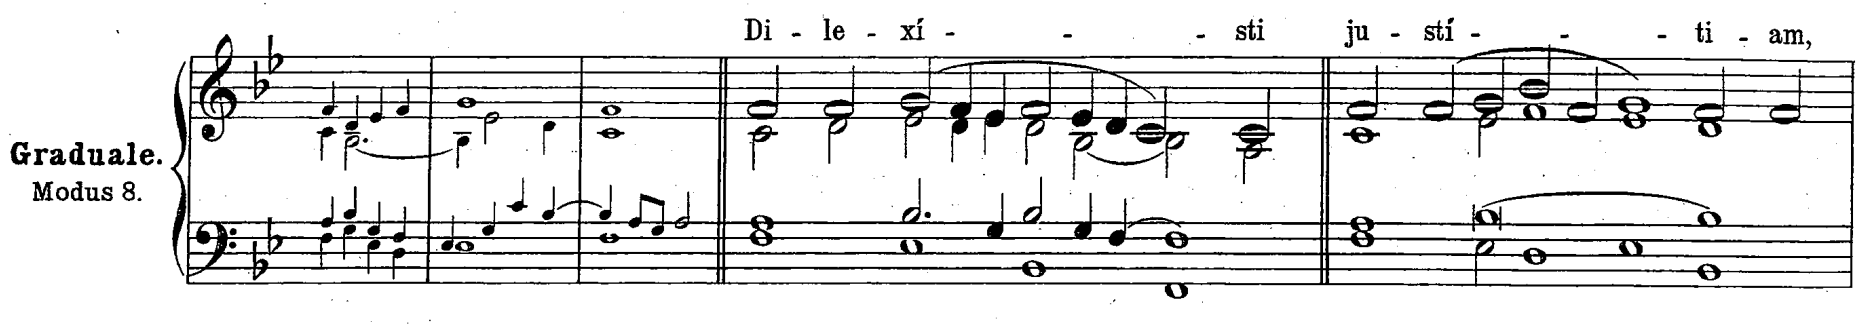
\includegraphics[width=.8\linewidth]{c/1/ex/schildknecht_supplement_[60].png}
    \caption{Schildknecht, Prelude, harmonised intonation and larger noteheads, 1892}
    \label{mus:schildknecht_supplement_[60]}
  \end{example}

  \vspace*{\fill}

\end{landscape}

\begin{landscape}

\vspace*{\fill}

  \begin{example}
    \centering
    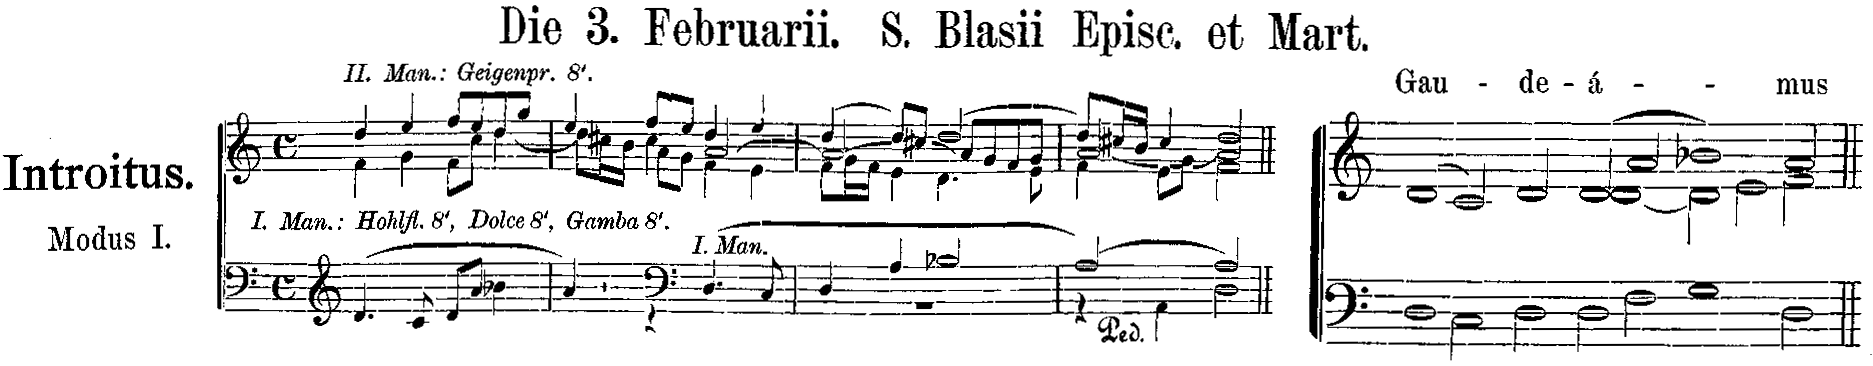
\includegraphics[width=.8\linewidth]{c/1/ex/quadflieg_supplement_(45).png}
    \caption{Quadflieg, Contrapuntal prelude and harmonised intonation, 1894}
    \label{mus:quadflieg_supplement_(45)}
  \end{example}

  \vspace*{\fill}

\end{landscape}

\begin{landscape}

  \vspace*{\fill}

  \begin{example}
    \centering
    \includegraphics[width=.7\linewidth]{c/1/ex/quadflieg_zaccaria_ap1.png}
    \caption{Quadflieg, Introit for the feast of St Anthony Maria Zaccaria, 1900}
    \label{mus:quadflieg_zaccaria_ap1}
  \end{example}

\vspace*{\fill}

\end{landscape}

\vspace*{\fill}

\begin{example}
  \centering
  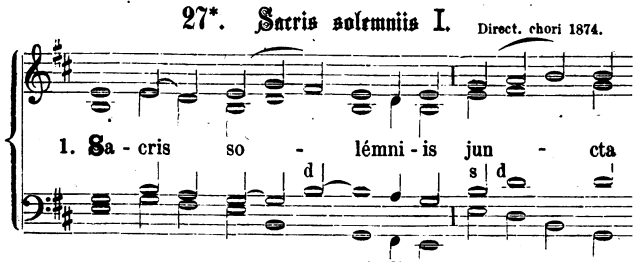
\includegraphics[width=.7\linewidth]{c/3/ex/piel_mohr_cantiones_56.png}
  \caption{Piel, Tenor part annotated with abbreviated \emph{dexter} and \emph{sinister}, 1878}
  \label{mus:mohrpiel_cantiones_56}
\end{example}

\vspace*{\fill}

\begin{landscape}

  \vspace*{\fill}

  \begin{example}
    \centering
    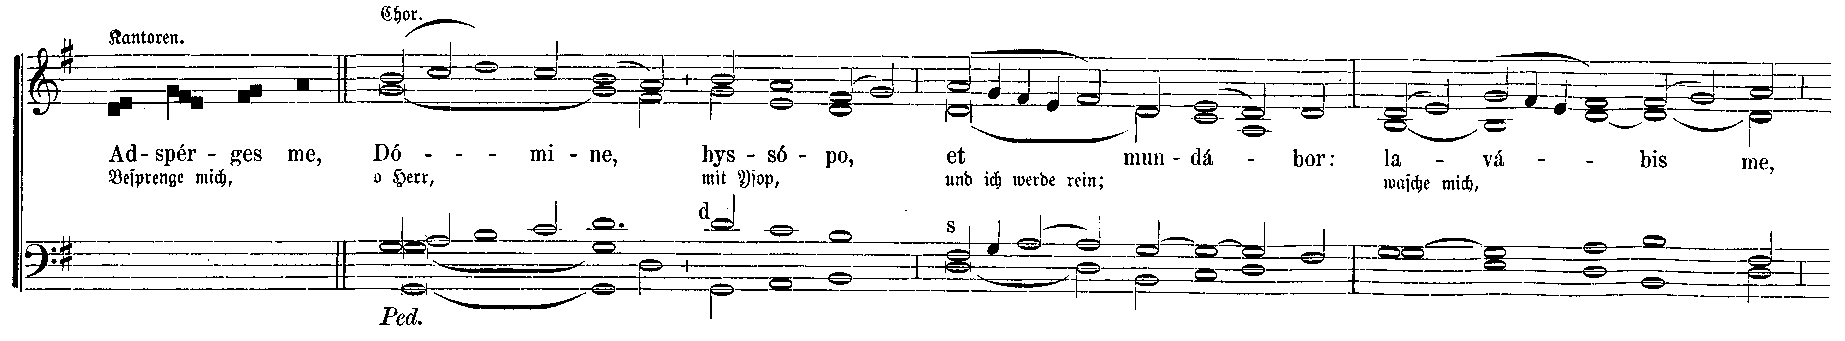
\includegraphics[width=\linewidth]{c/3/ex/piel_mohrordinarium_2.png}
    \caption{Piel, Intonation in quadratic notation, 1888}
    \label{mus:piel_mohrordinarium_2}
  \end{example}

  \vspace*{\fill}

\end{landscape}

\begin{landscape}

  \vspace*{\fill}

  \begin{example}
    \centering
    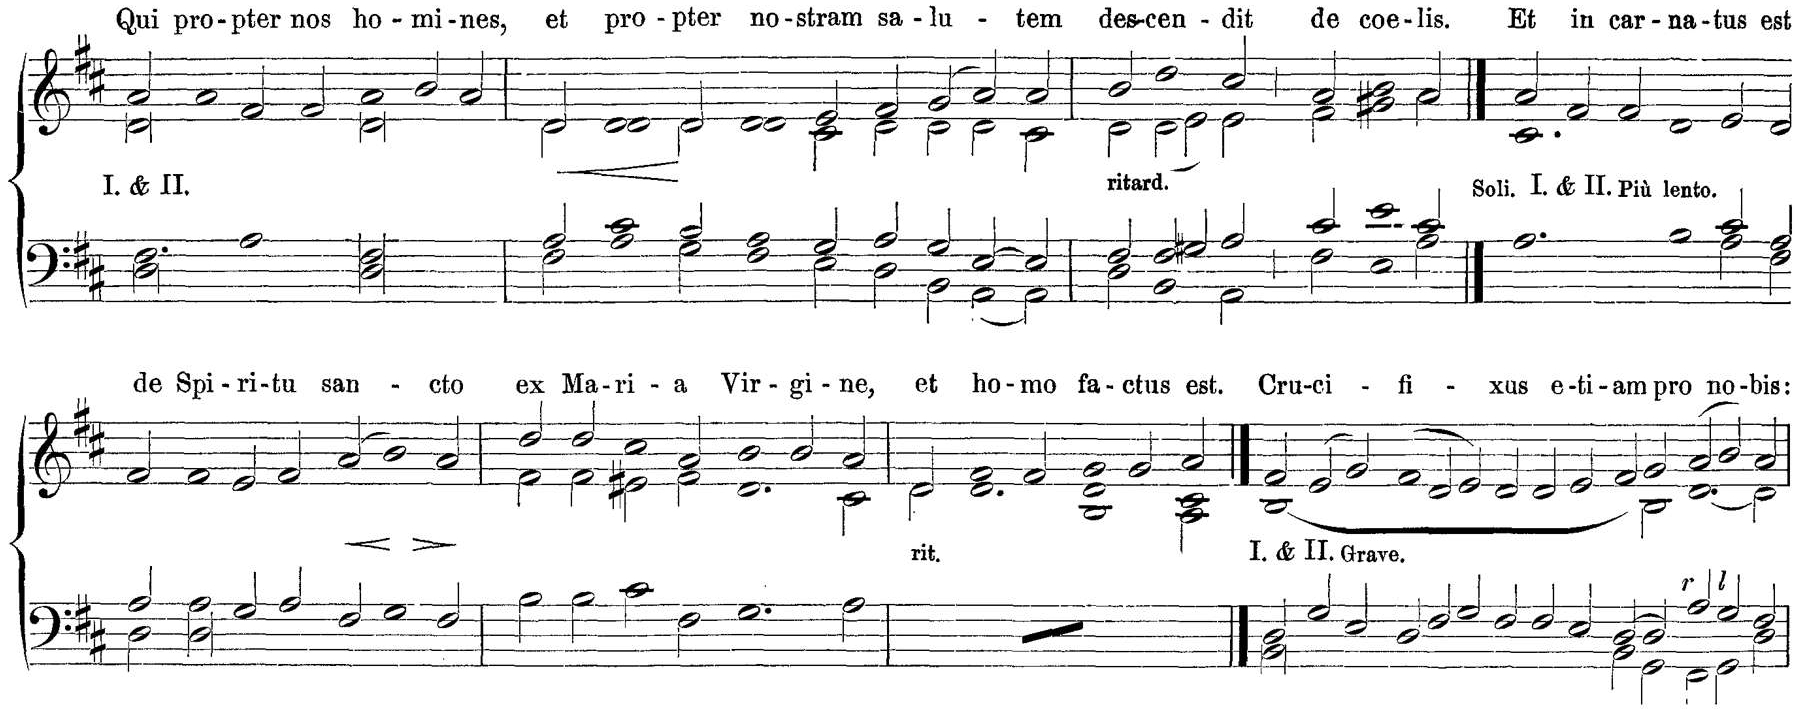
\includegraphics[width=.7\linewidth]{c/1/ex/willibald_20.jpeg}
    \caption{Wanger, Trappist accompaniment for South Africa, 1894}
    \label{mus:willibald_20}
  \end{example}

  \vspace*{\fill}

\end{landscape}

\vspace*{\fill}

\begin{example}
  \centering
  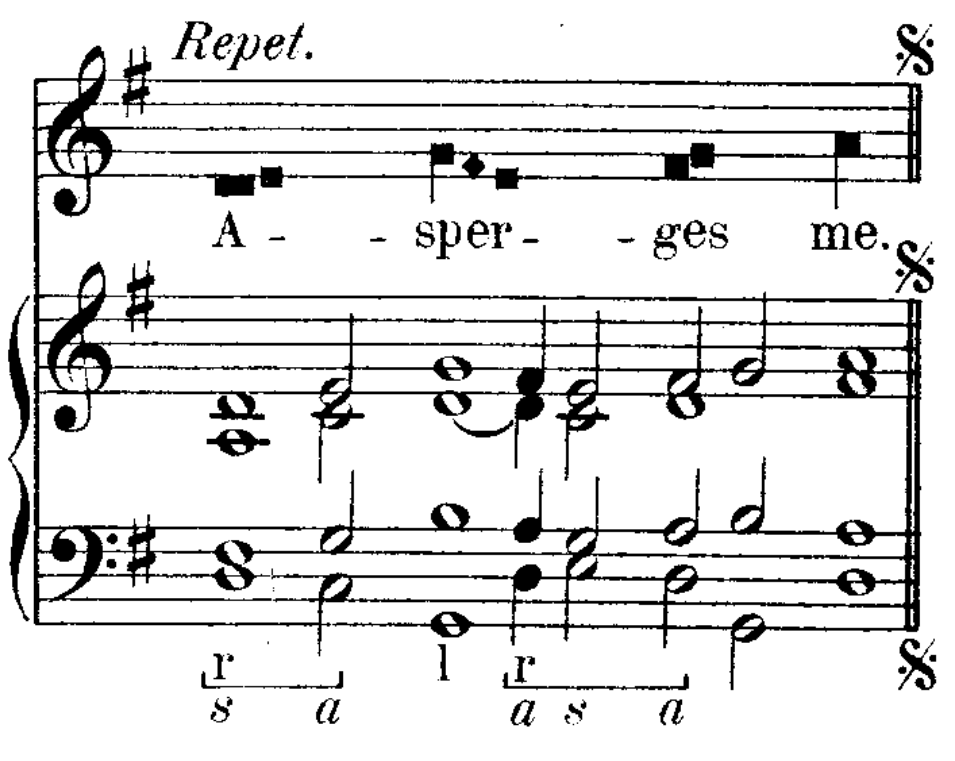
\includegraphics[width=.5\linewidth]{c/3/ex/habert.png}
  \caption{Habert, Annotated `Asperges me', \emph{c}.1885}
  \label{mus:habert}
\end{example}

\vspace*{\fill}


\begin{example}
  \centering
  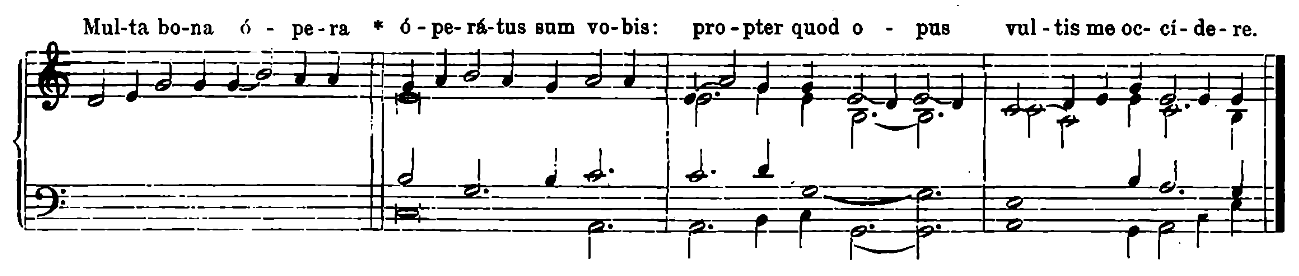
\includegraphics[width=\linewidth]{c/1/ex/orel_jirasek_66-7.png}
  \caption{Jirásek, Czech accompaniment, 1899}
  \label{mus:orel_jirasek_66-7}
\end{example}

\vspace*{\fill}

\newpage
